
%\section{TDNN}
\label{sec:application:tdnn}

For the implementation of the two kind of dynamic ANNs already described, 
\ie, the TDNN (\subsecref{ANN:TDNN}) and the NARX models (\subsecref{ANN:NARX}), 
we made used of the MatLab Toolbox for neural networks too. 

Since we can considered a TDNN as a NARX model with the same input TDL 
and a null delayed connection from the output to the input layer, 
the bulding process of both ANNs is practically equal. Hence, if the the previous values of the independent exogenous input signal $u(t)$ in the NARX model was denoted as $d_{u}$, we can expressed the same way the TDL time steps of the TDNN. For simplicity during the ANNs implementation, we denote this parameter as $n_{b}$. The delayed connection from the output to the input layer ($d_{y}$ in the NARX model), if exists, is from now expressed as $n_{a}$. 
Finally, the prediction horizon is denoted as $n_{k}$ as it happens with the feedforward networks (\subsecref{perceptronapplication}).

The most paramount aspect we must take into account is that samples cannot be introduced in the dynamic network the same way as with a static one. 
In the latter, all the samples of a entire time-window are presented to the network at a time, that is, samples are concurrent. 
In dynamic networks, only one sample of each time series is introduced every step, maintaining always the temporal order among samples. Therefore we must indicate the Toolbox that the network inputs are sequencial signals and not concurrent samples. With MatLab, this process is carried out using the cell format instead of the matrix one. Notice that also de output must be defined as a sequencial signal.

The turn of the screw is in the fact that we have a set of four concurrent physiological time series. Therefore, we must combined the matrix and the cell format in order to point out that samples are sequencial within their corresponding signal, but concurrent with the samples of the same time step of the other physiological time series.

The following sections expose the peculiarities and results of the Time Delay and NARX networks used.





\subsection{TDNN}
\label{subsec:tdnnapplication}

\figref{tdnnbuilt} shows an example of a TDNN built.
\begin{figure}[!ht]
\centering
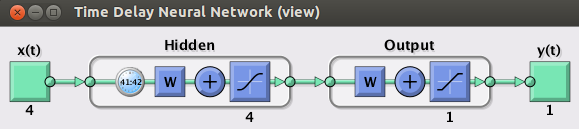
\includegraphics[width=0.9\columnwidth]{images/results/tdnn}
\caption{Example of a TDNN we have evaluated}
\label{fig:tdnnbuilt}
\end{figure}

From left to right, we can observe that it comprises a set of four input concurrent samples, 
one for each physiological signal (HR, EDA, TEMP, SpO2). This signals are formatted as sequencial in order to preserve its temporal characteristic.

The circle we found next represents the TDL. It consists of two numbers. The first one determined the prediction horizon $n_{k}=(41)-1=40$ (it is substracted $1$ because MatLab enumerates the time steps starting by $1$). The difference between the second number and the first one fixes the amount of input previous values used to compute the output, \ie, the memory of the system. Therefore, $n_{b}=(42-41)+1=2$ (it is added $1$ because the ends of the interval are also taken into account).

Both $n_{k}$ and $n_{b}$, as well as the number of physiological signals used, are modified and evaluated. Thus, we set the next experimental ranges: $n_{k}\in [10,40]$, $n_{b}\in [1,5]$. Greater values of $n_{k}$ improves the prediction, while if $n_{b}$ increases, more memory and computation capacities requires the ANN.

We observed that there are four neurons in the hidden layer -in fact, we configured the network to have the number of hidden neurons equals to the amount of physiological signals in the input layer. All of them have an hyperbolic tangent sigmoid as activation function. On the contrary, the unique output neuron has a symetric saturating linear function. These types of transfer function have been set after experimenting several alternatives. None of the layers have biases terms.

Althought the training phase presents an acceptable outcome (\figref{tdnntraining}), the test phase is always much worse (\figref{tdnntest}). This difference can be an evidence of overfitting of the training set, which is very common when the number of well-known patterns are ver low.

\begin{figure}[!ht]
\centering
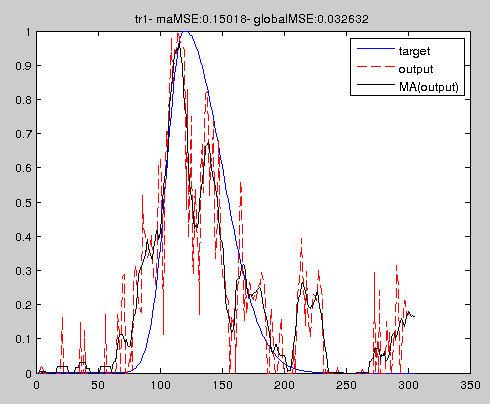
\includegraphics[width=0.7\columnwidth]{images/results/tdnnTraining}
\caption{Acceptable outcome of a TDNN while training}
\label{fig:tdnntraining}
\end{figure}

\begin{figure}[!ht]
\centering
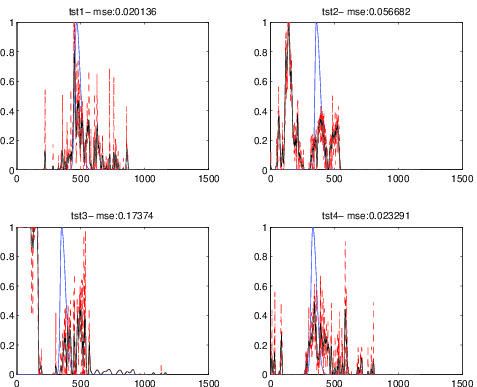
\includegraphics[width=0.9\columnwidth]{images/results/tdnnTest}
\caption{Non acceptable result of a TDNN in the test phase}
\label{fig:tdnntest}
\end{figure}

Notice that the original output of the network (red) is almost chaotic, but performing its 12-points moving average (MA), a more target-alike signal (blue) is obtained. However, with this test results, it is impossible to set threshold value with which we can conclude that a migraine is detected in advanced.




\subsection{NARX}
\label{subsec:narxapplication}



\begin{figure}[!ht]
\centering
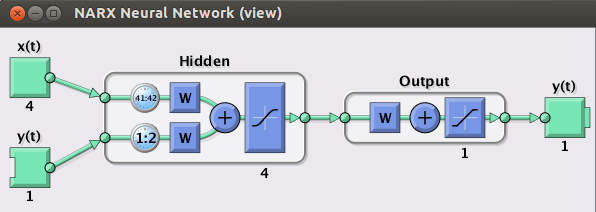
\includegraphics[width=0.9\columnwidth]{images/results/narxOpenloop}
\caption{Example of an openlooped NARX network we have evaluated}
\label{fig:narxopenloop}
\end{figure}


We implemented the NARX neural network with the Neural Network 
Toolbox of MatLab. In order to adapt the topology to our scenario, 
we configured the network with four exogenous inputs (HR, EDA, 
temperature and SpO2). We used as output signal of the system a line 
whose slope is determined by the time interval between the 
beginnings of the aura and pain phases. With this line we try to 
predict the upward slope of the symptomatic curve of probability we 
have just modelled. 

The used NARX network counts with one hidden layer with 10 
neurons apart from the input and output layers. 
The memory feature is included with a tapped delay line at input. 
The activation function of the hidden layer was established as 
a \textit{tansig}, whereas the one used in the output layer is 
a \textit{purelin}. Then, in order to obtained values in the range of [0,1], values lower than 0 were fixed to 0 and the ones greater than 1 to a value of 1.

Another consideration to take into account is that we trained the 
NARX network in open loop, in which the true output is used instead 
of feeding back the estimated output. The NARX network was then 
converted to the closed loop configuration for validating and 
testing the model.

The training set consists on one, two or three migraines and then we tested the model with the four migraines we had at our disposal. 
We iteratively checked the perform  
of the possible combinations of values of 
$n_{a}$, $n_{b}$ and $n_{k}$, where $n_{a} = n_{b}$ to reduce
complexity. As the weights of the neurons were randomly initialized,
we created several nets with the same configuration and initialized
and trained each one independently. Then, we compared the results
and stored the best one.

After checking iteratively the perform  
of the possible combinations of values of 
$n_{a}=n_{b}$ and $n_{k}$, with different training and testing
sets, the best NARX model with ANN was obtained when the net was 
trained with three migraines, with $n_{k}=10$ and $n_{a}=6=n{b}$.
In order to avoid false positives, we fixed a threshold 
of probability of detection of 0.5. The margin of prediction is then 
defined as the sum of the $n_{k}$ value and the time interval 
between the instant when the prectictive curve reaches the threshold 
and the begining of the aura. The resultant graphic 
(\figref{narxTest})
shows that we gain a range of 100-200 extra
minutes for predicting. In contrast, the system must be restarted
every time a migraine is detected since it maintains its high level 
response indefinitely. This would be one of the aspects to improve 
in further works.



\begin{figure}[!ht]
\centering
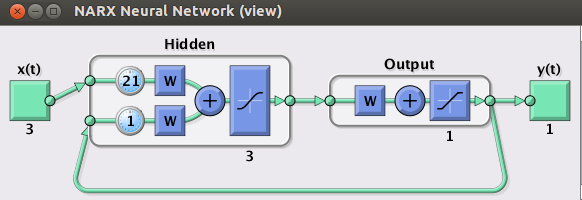
\includegraphics[width=0.9\columnwidth]{images/results/narxCloseloop}
\caption{The closeloop NARX network we have obtained the best test results with}
\label{fig:narxcloseloop}
\end{figure}




\begin{figure}
\centering
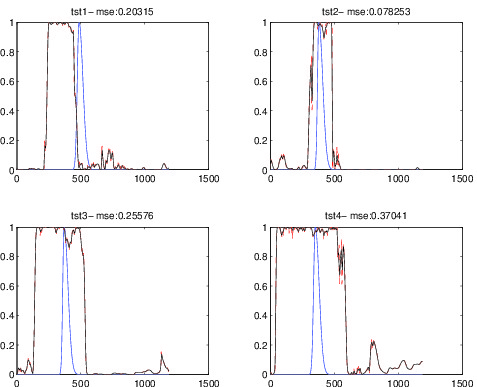
\includegraphics[width=\columnwidth]{images/results/narx_sinEDA_trn3_na-nb1-nk10_NN1}
\caption{NARX model test for the four migraines considered}
\label{fig:narxTest}
\end{figure}